\section{Otimização}
\label{sec:otimizacao_revbib}

Otimizar é escolher, dentro de um conjunto de possibilidades, os valores das
variáveis de decisão que tornam mínima (ou máxima) uma função que mede o
desempenho de um sistema \cite{nocedal2006numerical}. Na forma geral, o
problema é

\begin{equation}
    \mathbf{x}^{\star} = \arg\min_{\mathbf{x} \in \Omega} J(\mathbf{x}),
    \qquad \Omega = \{\mathbf{x} : \mathbf{x}_{min} \le \mathbf{x} \le \mathbf{x}_{max}\}
    \label{eq:problema_otimizacao}
\end{equation}

\noindent em que $\mathbf{x}$ é o vetor de variáveis de decisão, $J$ é a
função-custo (ou função objetivo) e $\Omega$ é a região de busca, aqui
definida por limites em cada variável. Quando $J$ é convexa, qualquer mínimo
local é também o mínimo global, e métodos baseados no gradiente convergem
rapidamente para ele. Quando $J$ é não convexa, com vários vales, o método pode
parar em um mínimo local que não é o melhor da região
\cite{nocedal2006numerical}. A \autoref{fig:convexa_naoconvexa} ilustra os dois casos.

\begin{figure}[H]
    \centering
    \caption{Função-custo convexa, com um único mínimo, e não convexa, com
    mínimos locais além do global.}
    \label{fig:convexa_naoconvexa}
    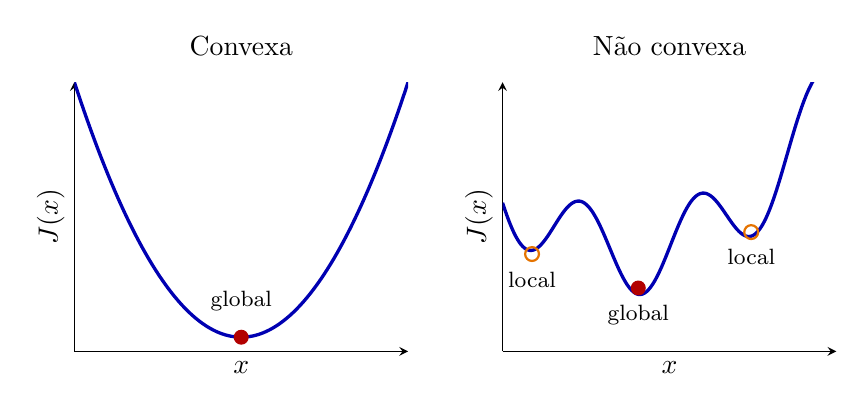
\begin{tikzpicture}
        \begin{axis}[name=a1, width=0.48\textwidth, height=5cm,
            xlabel={$x$}, ylabel={$J(x)$}, title={Convexa},
            xmin=-3, xmax=3, ymin=-0.5, ymax=9, ticks=none, axis lines=left]
            \addplot[blue!70!black, very thick, domain=-3:3, samples=100] {x^2};
            \addplot[only marks, mark=*, red!70!black, mark size=2.5pt] coordinates {(0,0)};
            \node[anchor=south, font=\footnotesize] at (axis cs:0,0.6) {global};
        \end{axis}
        \begin{axis}[at={(a1.east)}, anchor=west, xshift=1.2cm,
            width=0.48\textwidth, height=5cm,
            xlabel={$x$}, ylabel={$J(x)$}, title={Não convexa},
            xmin=-3, xmax=3, ymin=-2.5, ymax=4, ticks=none, axis lines=left]
            \addplot[blue!70!black, very thick, domain=-3:3, samples=200]
                {0.3*x^2 + sin(deg(3*x)) + 0.4*x};
            \addplot[only marks, mark=*, red!70!black, mark size=2.5pt] coordinates {(-0.56,-0.97)};
            \addplot[only marks, mark=o, orange!90!black, mark size=2.5pt, thick] coordinates {(1.47,0.38) (-2.47,-0.15)};
            \node[anchor=north, font=\footnotesize] at (axis cs:-0.56,-1.15) {global};
            \node[anchor=north, font=\footnotesize] at (axis cs:1.47,0.2) {local};
            \node[anchor=north, font=\footnotesize] at (axis cs:-2.47,-0.35) {local};
        \end{axis}
    \end{tikzpicture}

    \fonte{Autor (2026).}
\end{figure}


Em muitos problemas de engenharia, $J$ não tem expressão analítica: cada
avaliação exige simular o sistema com o candidato $\mathbf{x}$ e medir o
resultado. Nesse caso não há gradiente disponível, e estimá-lo por diferenças
finitas é caro e pouco confiável se a simulação tiver descontinuidades ou
regiões em que o sistema diverge. Para essa classe de problemas são usados
métodos livres de gradiente, que só precisam do valor de $J$. Entre os locais,
o mais conhecido é o simplex de \citeonline{nelder1965simplex}, que deforma um
conjunto de $n+1$ pontos em direção à região de menor custo. Entre os globais
estão os algoritmos evolutivos, que mantêm uma população de candidatos e a
fazem evoluir por operações inspiradas na seleção natural; a Evolução
Diferencial é um dos mais usados para variáveis contínuas
\cite{storn1997differential}.

\subsection{Evolução Diferencial}
\label{sec:evolucao_diferencial}

A Evolução Diferencial (\textit{Differential Evolution}, DE) mantém uma
população de $N_p$ vetores candidatos, inicialmente espalhados pela região de
busca \cite{storn1997differential}. Cada geração aplica três operações a cada
vetor $\mathbf{x}_i$:

\begin{itemize}
    \item \textbf{Mutação:} cria-se um vetor mutante a partir de três outros
    membros sorteados da população, $\mathbf{r}_1$, $\mathbf{r}_2$ e
    $\mathbf{r}_3$, com um fator de escala $F$:
    \begin{equation}
        \mathbf{v}_i = \mathbf{r}_1 + F\,(\mathbf{r}_2 - \mathbf{r}_3)
        \label{eq:de_mutacao}
    \end{equation}
    \item \textbf{Cruzamento:} forma-se um vetor de teste $\mathbf{u}_i$
    tomando cada componente de $\mathbf{v}_i$ com probabilidade $C_r$ e de
    $\mathbf{x}_i$ caso contrário;
    \item \textbf{Seleção:} $\mathbf{u}_i$ substitui $\mathbf{x}_i$ na geração
    seguinte apenas se $J(\mathbf{u}_i) \le J(\mathbf{x}_i)$.
\end{itemize}

\noindent A \autoref{fig:de_mutacao} ilustra a mutação em duas variáveis.

\begin{figure}[H]
    \centering
    \caption{Mutação da Evolução Diferencial em duas variáveis: o vetor
    diferença entre dois membros, escalado por $F$, é somado a um terceiro.}
    \label{fig:de_mutacao}
    \begin{tikzpicture}[scale=1.1, >={Latex}]
        % contornos de custo
        \foreach \r in {0.6,1.2,1.8,2.4,3.0}
            \draw[gray!40] (4,2.2) ellipse ({1.4*\r} and {0.8*\r});
        \fill[gray!60] (4,2.2) circle (1.5pt) node[below right, font=\scriptsize, gray] {mínimo};
        % populacao
        \foreach \p in {(0.6,0.6),(1.2,3.4),(6.8,0.5),(7.6,3.2),(2.4,4.0),(5.6,4.1)}
            \fill[black!50] \p circle (1.6pt);
        \coordinate (r1) at (1.6,1.0);
        \coordinate (r2) at (6.2,3.6);
        \coordinate (r3) at (3.4,4.3);
        \coordinate (xi) at (6.0,0.9);
        \fill[blue!70!black] (r1) circle (2pt) node[below left] {$\mathbf{r}_1$};
        \fill[blue!70!black] (r2) circle (2pt) node[above right] {$\mathbf{r}_2$};
        \fill[blue!70!black] (r3) circle (2pt) node[above left] {$\mathbf{r}_3$};
        \fill[black] (xi) circle (2pt) node[below right] {$\mathbf{x}_i$};
        \draw[->, thick, blue!70!black, dashed] (r3) -- (r2) node[midway, above, font=\footnotesize] {$\mathbf{r}_2 - \mathbf{r}_3$};
        \coordinate (vi) at ($(r1)+0.7*(r2)-0.7*(r3)$);
        \draw[->, very thick, red!70!black] (r1) -- (vi) node[midway, below, font=\footnotesize] {$F(\mathbf{r}_2 - \mathbf{r}_3)$};
        \fill[red!70!black] (vi) circle (2.2pt) node[above, font=\small] {$\mathbf{v}_i$};
        \draw[->, densely dotted, thick] (xi) -- node[right, font=\footnotesize, align=left] {cruzamento\\e seleção} ($(vi)!0.45!(xi)$);
        \node[font=\footnotesize] at (0.3,4.6) {$x_2$};
        \node[font=\footnotesize] at (8.2,0.0) {$x_1$};
        \draw[->] (0,0) -- (8.2,0); \draw[->] (0,0) -- (0,4.8);
    \end{tikzpicture}

    \fonte{Adaptado de \citeonline{storn1997differential}.}
\end{figure}


\subsection{Busca em Escala Logarítmica}
\label{sec:busca_log}

Variáveis de decisão de ordens de grandeza muito diferentes prejudicam a
busca, pois um mesmo passo é grande para uma e desprezível para outra. Uma
prática comum é otimizar o expoente: escreve-se cada variável como
$\Gamma_j = s_j\,10^{x_j}$, com sinal $s_j$ fixo, e a busca é feita sobre
$x_j$. Isso normaliza as escalas, de modo que um passo em $x_j$ corresponde a
uma variação relativa da variável, e impõe por construção o sinal de cada uma.

\subsection{Função-Custo e Métricas de Erro}
\label{sec:funcao_custo_revbib}

Quando o objetivo é que uma estimativa $\hat{y}_n$ siga um sinal de referência
$y_n$, a função-custo é construída a partir do resíduo $r_n = \hat{y}_n - y_n$
por uma métrica de erro \cite{hermuche2023funcoes, datacamp2025cost}. As mais
usadas são o erro absoluto médio (MAE), a raiz do erro quadrático médio (RMSE) e
a perda de Huber \cite{huber1964robust}:

\begin{equation}
    \mathrm{MAE} = \frac{1}{N}\sum_{n=1}^{N} |r_n|, \qquad
    \mathrm{RMSE} = \sqrt{\frac{1}{N}\sum_{n=1}^{N} r_n^2}, \qquad
    \ell_\delta(r) =
    \begin{cases}
        \tfrac{1}{2} r^2, & |r| \le \delta \\
        \delta\left(|r| - \tfrac{1}{2}\delta\right), & |r| > \delta
    \end{cases}
    \label{eq:metricas_erro}
\end{equation}

O MAE pesa todos os erros igualmente. O RMSE, por elevar o resíduo ao
quadrado, penaliza mais os erros grandes e tem a mesma unidade do sinal. A
perda de Huber é quadrática para resíduos pequenos e linear para os grandes, o
que a torna menos sensível a desvios esporádicos. A
\autoref{fig:metricas_erro_area} mostra, para os mesmos resíduos, a área que
cada métrica soma: no MAE cada resíduo contribui com uma faixa de altura
$|r_n|$; no erro quadrático, com um quadrado de lado $|r_n|$, de modo que o
resíduo grande domina a soma; na perda de Huber, os resíduos pequenos contam
como quadrados e o grande como uma faixa de largura $\delta$.

\begin{figure}[H]
    \centering
    \caption{Área somada por cada métrica de erro para os mesmos resíduos entre
    a referência $y_n$ e a estimativa $\hat{y}_n$: (a) erro absoluto, (b) erro
    quadrático e (c) perda de Huber.}
    \label{fig:metricas_erro_area}
    \begin{tikzpicture}[scale=0.55]
        % x_n / y_n (referência) / r_n (resíduo)
        \def\pontos{1/1.2/0.5, 2/1.8/-0.7, 3/2.4/0.4, 4/3.0/2.0, 5/3.6/-0.6, 6/4.2/0.7}
        \def\delt{0.8}
        \newcommand{\eixos}[1]{%
            \draw[->] (0,0) -- (7.8,0) node[below, font=\scriptsize] {$n$};
            \draw[->] (0,0) -- (0,6.0);
            \draw[thick, black!60] (0.5,0.9) -- (6.8,4.68);
            \node[font=\small] at (3.9,-1.0) {#1};}
        \newcommand{\pts}{%
            \foreach \x/\y/\r in \pontos {
                \pgfmathsetmacro{\yh}{\y+\r}
                \draw[densely dotted] (\x,\y) -- (\x,\yh);
                \fill[black] (\x,\y) circle (2.5pt);
                \fill[orange!90!black] (\x,\yh) circle (2.7pt);}}
        % (a) MAE
        \begin{scope}
            \eixos{(a) MAE}
            \foreach \x/\y/\r in \pontos {
                \pgfmathsetmacro{\yh}{\y+\r}
                \fill[blue!35, draw=blue!70!black] (\x-0.15,\y) rectangle (\x+0.15,\yh);}
            \pts
        \end{scope}
        % (b) RMSE
        \begin{scope}[xshift=9.3cm]
            \eixos{(b) RMSE}
            \foreach \x/\y/\r in \pontos {
                \pgfmathsetmacro{\yh}{\y+\r}
                \pgfmathsetmacro{\ar}{abs(\r)}
                \fill[red!25, draw=red!70!black, opacity=0.85] (\x,\y) rectangle (\x+\ar,\yh);}
            \pts
        \end{scope}
        % (c) Huber
        \begin{scope}[xshift=18.6cm]
            \eixos{(c) Huber}
            \foreach \x/\y/\r in \pontos {
                \pgfmathsetmacro{\yh}{\y+\r}
                \pgfmathsetmacro{\w}{min(abs(\r),\delt)}
                \fill[green!25, draw=green!50!black, opacity=0.85] (\x,\y) rectangle (\x+\w,\yh);}
            \pts
            \draw[<->, green!40!black] (4,5.35) -- node[above, font=\scriptsize] {$\delta$} (4.8,5.35);
        \end{scope}
        % legenda
        \fill[black] (7.5,-2.1) circle (2.5pt) node[right, font=\small] {referência $y_n$};
        \fill[orange!90!black] (15.0,-2.1) circle (2.7pt) node[right, font=\small] {estimativa $\hat{y}_n$};
    \end{tikzpicture}

    \fonte{Autor (2026).}
\end{figure}

Quando o custo soma termos de grandezas diferentes, como torque e velocidade,
cada resíduo é normalizado, por exemplo pelo desvio-padrão do sinal de
referência, e os termos são combinados por pesos. A métrica escolhida altera o
peso efetivo de cada termo: com a perda de Huber, um termo cujos resíduos
normalizados ficam abaixo de $\delta$ é comprimido em relação a outro que já
está no trecho linear, mesmo com pesos nominais iguais.
